\documentclass[11pt,a4paper]{article}
\usepackage[text={6.5in,10in},centering,a4paper]{geometry}
\usepackage{indentfirst}
\usepackage{setspace}
\usepackage{amssymb,amsmath} % Equations
\usepackage{tabularx} % Tables
\usepackage{graphicx,color} % Graphics, Figures
\usepackage[tight,footnotesize]{subfigure}
\usepackage{pgfgantt} % for gantt chart
\usepackage{hyperref}
\usepackage[titletoc]{appendix}
\usepackage[nottoc,numbib]{tocbibind}
\usepackage[numbers]{natbib}
\usepackage[no-math]{fontspec}
\usepackage{xunicode} % for Thai fonts
\usepackage{xltxtra} % for Thai fonts

\def\figurename{รูปที่}
\def\tablename{ตารางที่}
\def\refname{เอกสารอ้างอิง}
\def\chaptername{บทที่}
\def\abstractname{\large Abstract}
\def\contentsname{สารบัญ}
\def\listfigurename{สารบัญรูป}
\def\listtablename{สารบัญตาราง}
\def\figurename{รูป}
\def\tablename{ตาราง}
\def\appendixname{ภาคผนวก}

\graphicspath{{figures/}} % create a director 'figures' in your local dir and all pics are kept here

%========== Thai Font ===========================
\XeTeXlinebreaklocale "th_TH"
\defaultfontfeatures{Scale=1.0, Mapping=tex-text} 
\setmainfont[Scale=1.2]{THSarabunNew}
%========== Thai Font ===========================

\begin{document}
\thispagestyle{empty}
\begin{center}
\doublespacing
{\LARGE \bf รายงานeartasrtarโครงงานวิศวกรรมไฟฟ้า วิชา 2102499}
\vfill
{ 
\LARGE \bf
% ชื่อโครงงานภาษาไทย
การพยากรณ์ความเข้มแสงอาทิตย์สำหรับบริเวณจุฬาลงกรณ์มหาวิทยาลัยโดยใช้แบบจำลองอนุกรมเวลา \\[2ex]
% ชื่อโครงงานภาษาอังกฤษ
Solar Irradiance Forecasting for Chulalongkorn University Location Using Time Series Models
}
\vfill
{\LARGE \bf นายขยัน เรียนดี เลขประจำตัว XXXX}\\[2ex]
{\LARGE \bf อาจารย์ที่ปรึกษา ผศ.ดร. จิตโกมุท ส่งศิริ}
\vfill
{\LARGE \bf ภาควิชาวิศวกรรมไฟฟ้า คณะวิศวกรรมศาสตร์}\\[2ex]
{\LARGE \bf จุฬาลงกรณ์มหาวิทยาลัย}\\[2ex]
{\LARGE \bf ปีการศึกษา 25xx}
\end{center}

\newpage
\thispagestyle{empty}
\begin{center}
\textbf{บทคัดย่อ}
\end{center}

โครงงานนี้นำเสนอการพยากรณ์ความเข้มแสงอาทิตย์ด้วยแบบจำลองอนุกรมเวลา ซึ่งมีประโยชน์ต่อการนำไปใช้งานด้านการจัดการพลังงาน โครงงานนี้พิจารณาการหาแบบจำลอง การจัดการกับข้อมูลที่หายไปหรือความต่างกันของสเกลเวลาในข้อมูล การพัฒนาแบบจำลองที่คำนึงถึงข้อมูลที่มีเทรนด์ตามฤดู และการวิเคราะห์ผลจากตัวแปรทางอากาศที่เกี่ยวข้อง ในโครงงานนี้ได้จัดการข้อมูลที่หายไปด้วยการเติมค่าเฉลี่ยของความเข้มแสงที่ผ่านการแยกแยะตามสภาพภูมิอากาศ การแยกแยะนั้น ประกอบด้วยการแบ่งข้อมูลตามฤดู ซึ่งคำนวณจากการเปลี่ยนแปลงความชันของอุณหภูมิกับความชื้นสัมพัทธ์ และประกอบกับการใช้เอสวีเอ็ม สำหรับปัญหาเรื่องสเกลเวลาที่ต่างกันในข้อมูลแต่ละตัวแปร โครงงานนี้ได้ใช้การประมาณค่าในช่วงแบบสไปลน์เพื่อเติมค่าข้อมูลที่มีความถี่ชักตัวอย่างต่ำกว่าค่าความเข้มแสง สำหรับแบบจำลองนั้น โครงงานนี้ได้ใช้แบบจำลองอาริมาที่มีเทรนด์แยกฤดูและตัวแปรภายนอก การกำจัดเทรนด์นั้นใช้วิธีการหาอนุกรมฟูริเยร์ และผลการทดลองพบว่าตัวแปรทางสภาพอากาศซึ่งได้แก่ ความชื้นสัมพัทธ์ ความดันอากาศ อุณหภูมิ และความเร็วลมนั้น มีผลน้อยมากต่อคุณภาพของแบบจำลอง เราจึงสรุปว่าการใช้แบบจำลองอาริมาที่มีเทรนด์ฤดูจึงเหมาะสมกับการพยากรณ์ความเข้มแสงอาทิตย์

\paragraph{\textbf คำสำคัญ:} การตอบสนองความต้องการ, การควบคุมอุณหภูมิ (ใส่ 3-5 คำ คั่นด้วย comma)

\begin{center}
\textbf{Abstract}
\end{center}

This project considers a solar irradiance forecasting using time series models which finds an application in solar power prediction for energy management. The focuses of this project are on finding practical time series models for solar forecasting, proposing the effective approaches for missing-data and asynchronous sampled data issues, improving the models by removing seasonal trends from the historical data, and analyzing the effect of exogenous inputs which may be included in the models to improve the forecast. A time series prediction typically requires a complete set of historical data while the global horizontal irradiance (GHI) data in Thailand are frequently missing for consecutive days. This project proposes a data-missing imputation technique using the mean value of GHI averaged over the data corresponding to the same weather type. The required weather classification consists of two steps: a seasonal segmentation based on detecting changes of monotonic properties of temperature and humidity time series, and a nonlinear support vector machine (SVM) that uses weather labels from the previous seasonal segmentation. For asynchronous sampled data issue, the relevant variables in Thailand has the lower sampling rate than GHI. This project uses Spline interpolation to fill all data to be at the sampling rate. Autoregressive integrated moving average models (ARIMA) is considered in this project. To improve the accuracy, this project proposes two techniques for seasonal effect removal including Seasonal ARIMA models (SARIMA) and removal of seasonal trend fitted by Fourier Series. These models may be further improved if exogenous inputs are included in the models, known as ARIMA with Exogenous Variables (ARIMAX). Our studies found that other meteorological inputs which are relative humidity, air pressure, local temperature and wind speed marginally affect the accuracy of the forecast. At the end, we recommend to use SARIMA as the forecasting model based on a model selection criterion.

\paragraph{\textbf Keywords:} solar forecasting, ARIMAX models, Seasonal ARIMA, Fourier series, imputation (three to five)

\paragraph{\textbf หมายเหตุ:}
\begin{enumerate}
\item บทคัดย่อทั้งภาษาไทยและภาษาอังกฤษควรมีความยาวรวมกันไม่เกิน 1 หน้า
\item รายงานควรมีความยาวไม่เกิน 25 หน้า (ไม่รวมปก บทคัดย่อ สารบัญ กิตติกรรมประกาศ เอกสารอ้างอิง และภาคผนวก)
\end{enumerate}

\newpage
\thispagestyle{empty}
\tableofcontents

\newpage
\setcounter{page}{1}
\section{บทนำ}
\subsection{ที่มาและความสำคัญของโครงงาน}
หัวข้อนี้เป็นการกล่าวถึง ความเป็นมา เหตุผล หรือแรงจูงใจ ที่ทำให้นิสิตเลือกหัวข้อโครงงานนี้ และประโยชน์หรือความสำคัญของโครงงานนี้ต่อการพัฒนาองค์ความรู้ในด้านต่างๆ เช่น ในเชิงวิชาการ เชิงเศรษฐกิจ เชิงวิศวกรรม ไม่ใช่กล่าวถึงการพัฒนาตัวนิสิตหรือสิ่งที่นิสิตจะได้รับ นิสิตอาจนำเสนอข้อมูล เช่น สถิติ ตาราง กราฟ เป็นต้น เพื่อสนับสนุนเหตุผล และความสำคัญ นิสิตควรเขียนแยกแต่ละประเด็นเป็นย่อหน้า การเขียนต้องกระชับ เข้าประเด็นโดยไม่อ้อมค้อม ซึ่งรวมถึงทุกส่วนในรายงานนี้ด้วย ไม่ควรอธิบายสิ่งที่เยิ่นเย้อและเป็นสิ่งที่รู้กันอยู่แล้ว เช่น “การประหยัดพลังงานเป็นสิ่งสำคัญที่ทุกคนต้องคำนึงถึง” “ในอนาคตหุ่นยนต์จะมีบทบาทเข้ามาทำงานแทนมนุษย์อย่างสิ้นเชิง” หรือ “ในยุคดิจิตอลจะช่วยให้มนุษย์สื่อสารและทำงานได้มีประสิทธิภาพมากขึ้นหากมีโครงข่ายสื่อสารทั่วโลก”


ในส่วนถัดมาให้อธิบายว่าหัวข้อโครงงานที่เลือกทำนี้ มีประเด็นปัญหาสำคัญอะไรบ้าง มีรายละเอียดหรือลักษณะของปัญหาอย่างไร มีใครที่เคยแก้ปัญหาลักษณะนี้หรือคล้ายกันมาก่อนบ้าง ถ้าโครงงานนี้เป็นการต่อยอด หรือปรับปรุงผลงานจากโครงงานที่ทำมาก่อนหน้า หรือจากวรรณกรรม ควรต้องชี้ว่าผลงานเก่ามีจุดด้อย หรือจุดอ่อนอะไร และโครงงานนี้จะช่วยแก้ไข หรือปรับปรุงอะไร ในการกล่าวถึงงานที่ผู้อื่นได้ทำมาแล้ว จะต้องใส่เอกสารอ้างอิงให้ชัดเจน เช่น บทความที่กล่าวถึงเรื่อง XX พบได้ใน ~\cite{WaJ:08} การคัดลอกผลงานของผู้อื่น ไม่ว่าทั้งหมดหรือบางส่วน โดยไม่อ้างอิงแหล่งที่มา ถือเป็นการกระทำที่ผิดต่อศีลธรรมและจรรยาบรรณ หากพบว่านิสิตมีการกระทำดังกล่าว นิสิตจะได้รับเกรด U หรือ F


ย่อหน้าสุดท้าย ให้อธิบายถึงสิ่งที่คาดหวังว่าจะได้เมื่อจบโครงงาน (ไม่ใช่สิ่งที่ตัวนิสิตจะได้รับ) และวิธีการที่ใช้ หรือแนวทางการดำเนินการของโครงงานนี้โดยย่อ พร้อมแสดงถึงข้อดี หรือประเด็นที่นำเสนอใหม่ในโครงงานนี้ หากมีแผนผังความคิด (Mind Map) ที่จะช่วยให้เข้าใจโครงสร้างของโครงงานได้โดยง่าย ก็ขอให้ใส่ในหัวข้อนี้ด้วย ความยาวรวมของหัวข้อนี้ไม่ควรยาวเกินสองหน้า

\subsection{วัตถุประสงค์ของโครงงาน}
วัตถุประสงค์ คือผลลัพธ์สุดท้าย (Outcome) ของโครงงาน วัตถุประสงค์จะคล้ายกับหัวข้อโครงงาน เพียงแต่มีรายละเอียดและความชัดเจนมากกว่าหัวข้อ วัตถุประสงค์ควรเล็งถึงสิ่งที่เป็นรูปธรรม เช่น ออกแบบและสร้างอุปกรณ์ (Device) ประดิษฐ์หรือหาระเบียบวิธี (Algorithm) หาพารามิเตอร์หรือสภาวะที่เหมาะสม (Characterization or Optimization) ออกแบบและสร้างระบบ (System Integration) ศึกษาและเปรียบเทียบ (Study and Comparison) พัฒนาซอฟต์แวร์ (Software Development) วัตถุประสงค์ไม่ควรเป็นเพียงการกระทำ (Actions) ของนิสิต เช่น เรียนรู้การใช้โปรแกรม MATLAB/Simulink ศึกษาการใช้งานไมโครโปรเซสเซอร์ ทำความเข้าใจคณิตศาสตร์ เรียนรู้การใช้งานและทดสอบเครื่องมือ เป็นต้น นิสิตควรเขียนวัตถุประสงค์ให้กระชับ ไม่ควรยาวเกินหกบรรทัด และสามารถแยกเป็นข้อๆ เพื่อความชัดเจนได้ (ไม่ควรเกินสามข้อ) เช่น
\begin{enumerate}
\item เพื่อพัฒนาองค์ความรู้ด้าน XX 
\item เพื่อสร้างต้นแบบอุปกรณ์ XX ในการแก้ปัญหา YY
\item เพื่อพัฒนาชุดซอฟท์แวร์ XX ในการแก้ปัญหา YY 
\item เพื่อหาแนวทางในการ XX
\end{enumerate}

ตัวอย่างวัตถุประสงค์ของโครงงานหัวข้อ “การวิเคราะห์ผลกระทบของระบบผลิตไฟฟ้าจากพลังงานแสงอาทิตย์ที่มีต่อเสถียรภาพชั่วครู่ของระบบไมโครกริด”
\begin{enumerate}
    \item เพื่อวิเคราะห์ผลของระบบผลิตไฟฟ้าจากพลังงานแสงอาทิตย์ที่มีต่อเสถียรภาพชั่วครู่ของไมโครกริด ทั้งในสภาวะที่เชื่อมต่อกับกริดภายนอกและสภาวะแยกโดด
    \item เพื่อวิเคราะห์ปัญหาเสถียรภาพชั่วครู่ของไมโครกริดเมื่อเกิดการรบกวนขนาดใหญ่ขึ้นในระบบ
\end{enumerate}

รายละเอียดในส่วนวัตถุประสงค์โครงงานในวิชา 2102499 นั้นจะต้องตรงกับที่เสนอไว้ในข้อเสนอโครงงานวิชา 2102490 ทุกประการ ถ้าหากในระหว่างการสอบข้อเสนอโครงงาน คณะกรรมการได้มีความเห็นให้เพิ่ม ลด แก้ไข หรือเปลี่ยนแปลงวัตถุประสงค์ นิสิตก็จะต้องจะแก้ไขตามคำแนะนำของคณะกรรมการด้วย

\subsection{ขอบเขตของโครงงาน}
ขอบเขตของโครงงานไม่ใช่ภาพรวมของโครงงาน ดังเช่นในวัตถุประสงค์ แต่เป็นการบอกเงื่อนไข สภาวะแวดล้อมที่ถูกสมมุติขึ้นสำหรับปัญหา รวมถึงผลลัพธ์ที่คาดหวังว่า จะมีขอบเขตอย่างไรที่วัดได้ โดยแยกเป็นข้อๆ แต่ละข้อต้องเป็นรูปธรรมที่ชัดเจน และต้องสามารถชี้วัดได้ในเชิงปริมาณไม่ใช่เชิงคุณภาพ เช่น เร็ว ควรเปลี่ยนเป็น อัตราอย่างน้อย 20 bps มีประสิทธิภาพสูง ควรเปลี่ยนเป็น ประสิทธิภาพอย่างน้อย 60 เปอร์เซ็นต์ เป็นต้น
ตัวอย่างขอบเขตของโครงงาน
\begin{enumerate}
    \item โครงงานนี้พิจารณาศึกษาระบบ XX ภายใต้สภาวะ YY เท่านั้น และจะทดลองในกรณีศึกษาทั้งหมด N กรณี ได้แก่ กรณี A กรณี B และกรณี C
    \item โครงงานนี้จะพัฒนาอุปกรณ์ XX ต้นแบบที่มีข้อกำหนด (Specification) ดังนี้ ข้อกำหนด A ข้อกำหนด B และข้อกำหนด C
\end{enumerate}

ตัวอย่างขอบเขตของโครงงานหัวข้อ “เครื่องตรวจจับระดับความเป็นกรดด่างของน้ำในสระว่ายน้ำ”
\begin{enumerate}
    \item ใช้หลักการตรวจจับการเปลี่ยนแปลงความเข้มแสงย่านแสงสีแดง
    \item สามารถใช้กับสระว่ายน้ำที่ต้องเติมคลอรีน ที่มีขนาดไม่เกิน 400 ลบ.ลิตร
    \item สามารถวัดค่าความเป็นกรดด่างได้ในช่วง pH 6.5-7.5 โดยมีความผิดพลาดไม่เกิน ±0.05
    \item สามารถตรวจจับได้อย่างรวดเร็ว โดยมีเวลาตอบสนองไม่เกิน 2 ms
\end{enumerate}

ขอบเขตของโครงงานในรายงานวิชา 2102499 นั้นจะต้องตรงกับที่เสนอไว้ในข้อเสนอโครงงานวิชา 2102490 โดยนิสิตสามารถเพิ่มขอบเขตได้ แต่ห้ามลดลง หากในระหว่างการสอบข้อเสนอโครงงาน คณะกรรมการได้มีความเห็นให้เพิ่ม ลด แก้ไข หรือเปลี่ยนแปลงขอบเขต นิสิตก็จะต้องแก้ไขตามคำแนะนำของคณะกรรมการด้วย

\subsection{ผลลัพธ์ที่คาดหวังจากโครงงาน}

ให้นิสิตอธิบายถึงผลลัพธ์ที่เป็นรูปธรรมที่ชัดเจนจากการทำโครงงานนี้ โดยเลือกเฉพาะผลลัพธ์ที่เด่นและเป็นผลลัพธ์หลัก เช่น

\begin{enumerate}
    \item ชุดซอฟท์แวร์ที่รับรูปภาพถ่ายของตา และแยกแยะได้ว่ามีอาการเสื่อมของโรคต้อกระจกตาหรือไม่
    \item ชุดคำสั่งตัวควบคุมเชิงทำนายแบบจำลอง (Model Predictive Control หรือ MPC) ด้วยภาษา XX ที่ใช้ควบคุมระบบ YY ตามเวลาจริง (Real time)
    \item รูปแบบปัญหาทางคณิตศาสตร์เพื่อประมาณหาแบบจำลองของระบบ XX พร้อมทั้งชุดคำสั่งเชิงเลขในการแก้ปัญหา
\end{enumerate}

ตัวอย่างผลลัพธ์ที่คาดหวังจากโครงงานหัวข้อ “การจำลองระบบทดสอบสำหรับใช้ศึกษาปัญหาเสถียรภาพชั่วครู่ในระบบส่งไฟฟ้ากำลัง”


ระบบทดสอบที่สามารถนำไปใช้ศึกษาและวิเคราะห์ปัญหาเสถียรภาพชั่วครู่ได้อย่างถูกต้อง


ผลลัพธ์ของโครงงานในวิชา 2102499 จะต้องตรงกับที่เสนอไว้ในข้อเสนอโครงงานวิชา 2102490 ห้ามลดมาตรฐานลง ถ้าในระหว่างการสอบข้อเสนอโครงงาน คณะกรรมการได้มีความเห็นให้ปรับปรุงผลลัพธ์ของโครงงาน นิสิตก็จะต้องแก้ไขตามความเห็นของคณะกรรมการด้วย

\section{หลักการและทฤษฎีที่เกี่ยวข้อง}
ในการทำโครงงานนั้น ย่อมต้องมีการใช้หลักวิชาความรู้ทางวิศวกรรมซึ่งอาจจะเป็นหลักการพื้นฐานที่นิสิตเคยเรียนมาแล้ว หรืออาจจะเป็นหลักการเรื่องใดเรื่องหนึ่งที่นิสิตต้องศึกษาเพิ่มเติม ความมุ่งหมายของหัวข้อส่วนนี้ คือการปูพื้นฐานทฤษฎีให้ผู้อ่านสามารถติดตาม และทำความเข้าใจโครงงานได้ เนื้อหาที่ไม่ควรใส่คือ หลักการหรือทฤษฎีทั่วไปที่อยู่ในตำราพื้นฐาน และไม่เกี่ยวข้องโดยตรงกับโครงงาน แม้ในกรณีที่มีความเกี่ยวข้องก็ไม่จำเป็นต้องอธิบายโดยละเอียด เหมือนการลอกมาจากตำรา สิ่งที่นิสิตควรอธิบายคือ หลักการหรือทฤษฎีขั้นสูง หรือการต่อยอดมาจากทฤษฎีพื้นฐาน ตัวอย่างเช่น งานที่เกี่ยวกับการประมวลผลสัญญาณ (Signal Processing) อาจมีการกล่าวถึงหลักการวิเคราะห์สเปกตรัม (Spectral Analysis)~\cite{StM:97} นิสิตควรต้องระบุและอธิบายถึงหลักการและทฤษฎีที่จะนำมาใช้ในโครงงาน ไม่ว่าจะเป็นสมการ ตาราง กราฟ สถิติ ขั้นตอน วิธีการ วงจร ระบบ อุปกรณ์ ฯลฯ แต่ไม่ควรนำสิ่งเหล่านี้มาแปะไว้เฉยๆ โดยไม่มีคำอธิบาย หรืออธิบายน้อยมาก นิสิตควรชี้ให้เห็นชัดเจนว่าหลักการและทฤษฎีต่างๆ จะถูกนำไปใช้อย่างไร การประยุกต์ใช้ทฤษฎีเพื่อแก้ปัญหาที่กำหนดขึ้นจะต้องมีความถูกต้องและเหมาะสมในเชิงวิศวกรรม เช่น ใช้สมการคณิตศาสตร์ที่ถูกต้อง เลือกใช้เทคนิคและเครื่องมือ (เช่น ซอฟต์แวร์) ที่จะนำมาใช้แก้ปัญหาทางวิศวกรรมได้อย่างเหมาะสม เป็นต้น


การเขียนควรเรียบเรียงเนื้อหาให้ต่อเนื่อง สั้นและกระชับแต่ได้ใจความ ความยาวโดยรวมไม่ควรเกินสิบหน้า การเขียนสามารถแยกเป็นหัวข้อย่อยได้ตามความเหมาะสม เนื่องจากรายงานโครงงานนี้เป็นงานเขียนทางวิชาการ การเขียนจะต้องเป็นไปตามหลักการเขียนงานทางวิทยาศาสตร์ เช่น การใช้ตัวแปรต้องมีความคงเส้นคงวา (Consistency) การอ้างสมการและการเลือกใช้สัญลักษณ์ ควรเป็นไปตามนิยม (Conventional) และไม่สับสน ภาษาที่ใช้ต้องเป็นภาษาเขียน ไม่ใช้ภาษาพูด การเขียนไม่ควรใช้ภาษาไทยสลับกับภาษาอังกฤษ ถ้ามีศัพท์ภาษาอังกฤษให้พยายามหาคำไทยที่นิยมใช้ (จากราชบัณฑิตยสภา หรือแหล่งอื่นๆ เป็นต้น) หรือพิจารณาเขียนทับศัพท์ แล้ววงเล็บศัพท์ภาษาอังกฤษไว้ข้างหลัง เฉพาะครั้งแรกที่พบศัพท์คำนี้ในรายงานเท่านั้น หากนิสิตต้องการศึกษาแนวทางเพิ่มเติม ในการเขียนบทความหรือรายงานทางวิทยาศาสตร์โดยใช้ภาษาไทย ขอแนะนำให้นิสิตอ่านหนังสือ ภาษาไทยสำหรับงานเขียนทางวิทยาศาสตร์และเทคโนโลยี โดย ศ.ดร.มงคล เดชนครินทร์


ในรายงานทั้งหมดจะต้องมีการอ้างอิงในรูปแบบที่ถูกต้อง ขอให้ดูตัวอย่างการอ้างอิงที่อยู่ท้ายตัวอย่างรายงานนี้ ข้อแนะนำคือ พยายามหลีกเลี่ยงการอ้างอิงสิ่งที่อยู่บนอินเตอร์เน็ต เพราะหน้าเว็บไซต์อาจมีการเปลี่ยนแปลงได้ตลอดเวลา ทำให้อาจไม่พบข้อมูลนั้นๆ เมื่อต้องการกลับมาดูอีก ถ้าเป็นไปได้ควรจะแทนด้วยสิ่งพิมพ์เช่น หนังสือ วารสาร บทความ รายงาน ฯลฯ ที่ให้สาระเหมือนกัน นอกจากนี้นิสิตควรใช้ Microsoft Word ในการเรียงลำดับรูป ตาราง สมการ และเอกสารอ้างอิงแบบอัตโนมัติด้วย

\section{ผลลัพธ์ของโครงงานและการอภิปรายผล}
จากหัวข้อผลลัพธ์ที่คาดหวังของโครงงานนั้น ในหัวข้อนี้ให้แสดงให้เห็นว่า สิ่งที่คาดหวังดังกล่าวได้บรรลุครบทุกข้อหรือไม่ และแสดงได้ด้วยผลการทดลอง การทดสอบระบบ หรือการวิเคราะห์อย่างไร โดยนำเสนอผลลัพธ์ในแต่ละขั้นตอนการดำเนินงานและผลลัพธ์สุดท้าย ผลการทดลองหรือการทดสอบต้องครบถ้วนสอดคล้องกับวัตถุประสงค์ที่ตั้งไว้ ทั้งนี้ให้อธิบายสมมติฐาน ระบบที่จำลอง (ถ้ามี) พารามิเตอร์ของส่วนประกอบต่างๆในการจำลองระบบให้ครบถ้วน และแสดงผลการทดลองในรูปแบบตารางและกราฟ ก่อนนำเสนอผลการทดลอง ขอให้นิสิตอธิบายโดยภาพรวมก่อนด้วยว่า ผลการทดลองที่เสนอนั้น มีกี่การทดลอง แต่ละการทดลองต้องการจะตอบคำถามใด และคาดหวังผลอย่างไรจากการทดลองนั้น เมื่อนำเสนอผลการทดลองแล้ว ให้อธิบายว่าเป็นไปตามที่คาดหรือไม่ และเพราะอะไร (ต้องมีเหตุผลทางทฤษฎีมาสนับสนุนด้วย) นิสิตควรเลือกนำเสนอผลลัพธ์ที่สำคัญและเกี่ยวข้องกับโครงงานที่ทำ ไม่ควรแสดงจำนวนการทดลองมากและเยิ่นเย้อโดยไม่จำเป็น เช่น การปรับค่าพารามิเตอร์หนึ่งๆ ในผลการจำลอง แล้วดูว่าส่งผลอย่างไร ขอให้ แสดงผลเฉพาะการปรับค่าพารามิเตอร์ที่จำเป็นเท่านั้น ในหัวข้อนี้ นิสิตอาจจะแบ่งเป็นหัวข้อย่อย (ตามผลการทดลอง หรืออย่างไรก็แล้วแต่) ตามความเหมาะสม


ขอให้นิสิตใส่ใจกับความชัดเจนของข้อมูล กราฟทุกกราฟ ตารางทุกตาราง เมื่อพิมพ์รายงานลงบนกระดาษขาวดำแล้ว ต้องสามารถอ่านได้ แยกเส้นกราฟได้ อ่านคำอธิบายกราฟ (Legend) ได้ มีคำกำกับแกนและคำอธิบายรูปกราฟชัดเจน รูปกราฟควรใช้เป็นแบบเวกเตอร์ (Vector Graphic) เนื่องจากรูปแบบเวกเตอร์จะสามารถยืดขยายได้ ไม่เหมือนกับรูปไบนารี่ (Binary) ที่เก็บรายละเอียดแบบพิกเซล (Pixel) ซึ่งจะเสียความละเอียด (Resolution) ไปเมื่อขยายรูปให้ใหญ่ขึ้น ถ้าใช้โปรแกรม MATLAB ในการวาดกราฟ ไม่ควรบันทึกรูปเป็นไฟล์ JPG แล้วนำมาวางในรายงานบนโปรแกรม Microsoft Word เพราะจะได้รูปที่ไม่คมชัด ให้นิสิตใช้คำสั่ง Copy Figure ซึ่งอยู่ในเมนู Edit ของหน้าต่างรูปกราฟของโปรแกรม MATLAB แล้วจึงนำมาวางในรายงาน จะได้รูปที่ชัดเจนกว่า หากข้อมูลเป็นตาราง ในส่วนของคำอธิบายตารางต้องบอกให้ชัดเจนว่า ตัวเลขในตารางคืออะไร หน่วยอะไร ควรมีการเน้นตัวเลขในตารางเพื่อให้ผู้อ่านสังเกตความแตกต่างได้โดยง่าย


สิ่งที่สำคัญสุดท้าย คือการอภิปรายและวิเคราะห์ผลการทดลอง ว่าเป็นไปตามสมมติฐานที่ได้หรือไม่อย่างไร โดยอธิบายตามหลักทฤษฎีที่ได้อ้างไว้ในหัวข้อหลักการและทฤษฎีที่เกี่ยวข้อง ขอให้นิสิตเข้าใจด้วยว่า การวิเคราะห์ผลการทดลองไม่ใช่การอ่านผลการทดลองหรือการอ่านกราฟ แต่เป็นการให้เหตุผลว่า ผลการทดลองที่ได้นั้นเป็นไปตามทฤษฎีหรือสมมติฐานที่ตั้งไว้หรือไม่อย่างไร นิสิตอาจจะเขียนอภิปรายเป็นส่วนหนึ่งในหัวข้อย่อยที่กล่าวถึงผลลัพธ์ของโครงงานแต่ละอย่าง หรือจะตั้งเป็นหัวข้อย่อยแยกต่างหากในหัวข้อนี้ก็ได้เช่นกัน


หากโครงงานของนิสิตมีการทดลอง ขอให้อภิปรายผลการทดลอง โดยมีหลักการทางวิทยาศาสตร์หรือวิศวกรรมมาสนับสนุน เช่น อภิปรายเปรียบเทียบผลของพารามิเตอร์ต่างๆ ในการทดลอง โดยมีเหตุผลทางทฤษฎีมาประกอบ


สำหรับโครงงานของนิสิตที่อาจจะไม่ได้มีผลการทดลองเพื่อตอบคำถามวิจัยใดๆ เช่น อาจจะเป็นการพัฒนาโปรแกรม หรือการพัฒนาต้นแบบ หรือการศึกษามาตรฐานใดแบบหนึ่ง ขอให้เขียนหัวข้อนี้เป็นการวิเคราะห์วิจารณ์ผลลัพธ์ของโครงงานที่ได้ว่าเป็นอย่างไร ใช้งานอุปกรณ์ต้นแบบแล้วได้ผลเป็นอย่างไร ผลเป็นไปตามที่คาดหวังหรือไม่ เนื่องจากเหตุผลใด

\section{บทสรุป}
\subsection{สรุปผลการดำเนินการ}
ให้นิสิตเขียนสรุปผลลัพธ์ของโครงงานให้ชัดเจน โดยอธิบายประโยชน์และแนวทางการนำโครงงานไปใช้งานในอนาคต ให้อภิปรายว่าโครงงานได้บรรลุวัตถุประสงค์สำเร็จตามขอบเขตที่ได้กำหนดไว้หรือไม่ อย่างไร บทสรุปไม่ควรมีเนื้อความที่เหมือนกับบทคัดย่อ

\subsection{ปัญหา อุปสรรค และแนวทางแก้ไข (ถ้ามี)}
ในหัวข้อนี้ ให้นิสิตกล่าวถึง ปัญหาและอุปสรรคที่ได้พบระหว่างการดำเนินงานมาจนถึงปัจจุบัน และให้อธิบายว่านิสิตได้หลบเลี่ยงหรือแก้ไขปัญหาอย่างไรบ้าง เช่น ถ้าต้องมีการเปลี่ยนแปลงวิธีการ เงื่อนไข หรือผลลัพธ์ที่ตั้งใจไว้แต่แรก ควรบอกว่าด้วยเหตุผลอะไร และควรมีข้อมูลมารองรับการตัดสินใจนั้นๆ ด้วย

\subsection{ข้อเสนอแนะ (ถ้ามี)}
ในส่วนนี้ ให้นิสิตเสนอแนะสิ่งที่ควรพิจารณาและดำเนินการต่อไปในอนาคต เช่น ควรจะศึกษาผลของปัจจัยใดเพิ่มเติม ควรจะปรับเปลี่ยนวิธีการทำโครงงานอย่างไร ควรจะพิจารณาปรับเปลี่ยนพารามิเตอร์ใดในการทดลอง หรือควรจะแก้ไขข้อบกพร่องของอุปกรณ์ต้นแบบอย่างไร

\section{กิตติกรรมประกาศ (ถ้ามี)}
หากนิสิตต้องการเขียนคำขอบคุณแหล่งทุนสนับสนุนการทำโครงงาน อาจารย์ที่ปรึกษา กรรมการสอบโครงงาน นิสิตรุ่นพี่ เพื่อน หรือรุ่นน้อง ให้เขียนคำขอบคุณไว้ที่ส่วนนี้ ทั้งนี้การอ้างถึงชื่อแหล่งทุนให้เขียนชื่อเต็ม ส่วนการอ้างถึงชื่อบุคคลอื่นให้ใช้ชื่อจริงพร้อมนามสกุลและคำนำหน้า

\section{ตัวอย่างคำสั่งที่ใช้งานใน LaTeX}
ในส่วนนี้จะแสดงตัวอย่างการใช้คำสั่ง LaTeX เบื้องต้น สำหรับ tutorial นั้นมีมากมายบน Internet ตัวอย่างเอกสารประกอบการใช้งาน LaTeX ภาษาไทยที่ดีอันหนึ่งคือจาก อ.ดร. ฑิตยา หวานวารี~\cite{cuthesis} เป็น template สำหรับวิทยานิพนธ์ของจุฬาลงกรณ์มหาวิทยาลัย แต่ได้อธิบายการใช้คำสั่งเบื้องต้นไว้โดยละเอียด

\subsection{การใส่ตาราง}
\begin{table}[ht]
\centering
\caption{ตัวอย่างตาราง} 
\vspace{3mm}
\begin{tabular}{|l|c|c|r|} \hline
Item & Font & Font Type & Font Size \\ \hline
Title & Garamond & Bold & 20 \\
Author names & Garamond & Bold & 12 \\ 
Author affiliation/email & Garamond & Regular & 11 \\
Abstract/Keywords & Garamond & Regular & 11 \\
Level 1 headings & Garamond & Bold & 12 \\
Level 2 headings & Garamond & Bold & 11 \\
Level 3 headings & Garamond & Regular & 11 \\
Figure/table captions & Garamond & Regular & 11 \\
Main text/References & Garamond & Regular & 11 \\ \hline
\end{tabular}
\end{table}

\subsection{การใส่รูป}
การใช้รูปในงานที่ compile ด้วย \XeLaTeX จะใช้รูป format .eps, .pdf, .jpg, .png เป็นต้น ขอให้ใช้ vector graphic เป็นหลัก สำหรับรูปผลการทดลองหรือการวาดแผนผังต่างๆ เนื่องจากรูปแบบเวคเตอร์จะสามารถยืดขยายได้ไม่เหมือนกับรูป binary ที่เก็บรายละเอียดแบบ pixel และจะมีการเสีย resolution ไปหากขยายรูป zoom ให้ใหญ่ขึ้น
\begin{figure}[ht]
	\begin{center}
		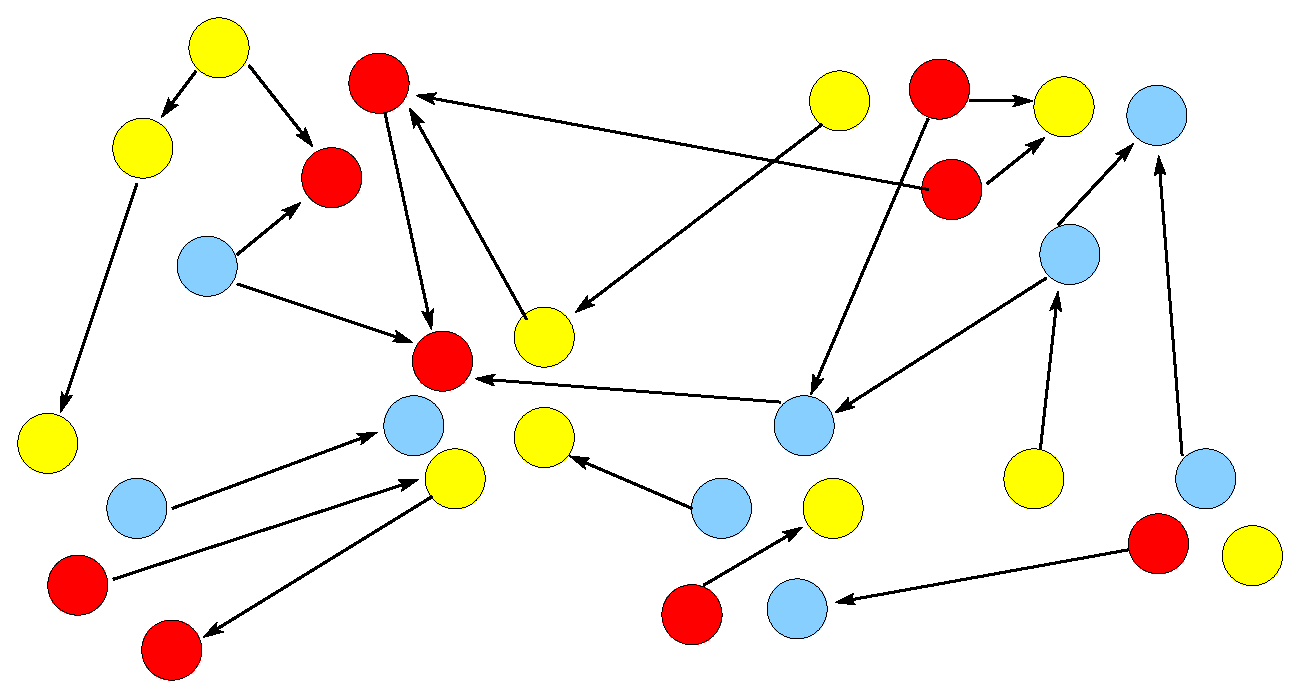
\includegraphics[width=0.7\linewidth]{gm.eps}
		\caption{แบบจำลองเชิงกราฟ}
	\end{center}
\end{figure}

\begin{figure}[h!]
	\begin{center}
		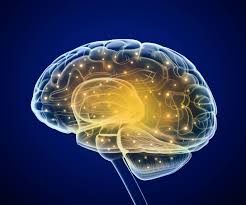
\includegraphics[width=0.5\linewidth]{brain.jpg}
		\caption{สภาพการเชื่อมโยงของสมอง (ที่มา: Shutterstock.com รูปโดย: Alex Mit)}
	\end{center}
\end{figure}

\begin{figure}
\centering
\subfigure[first caption]{ 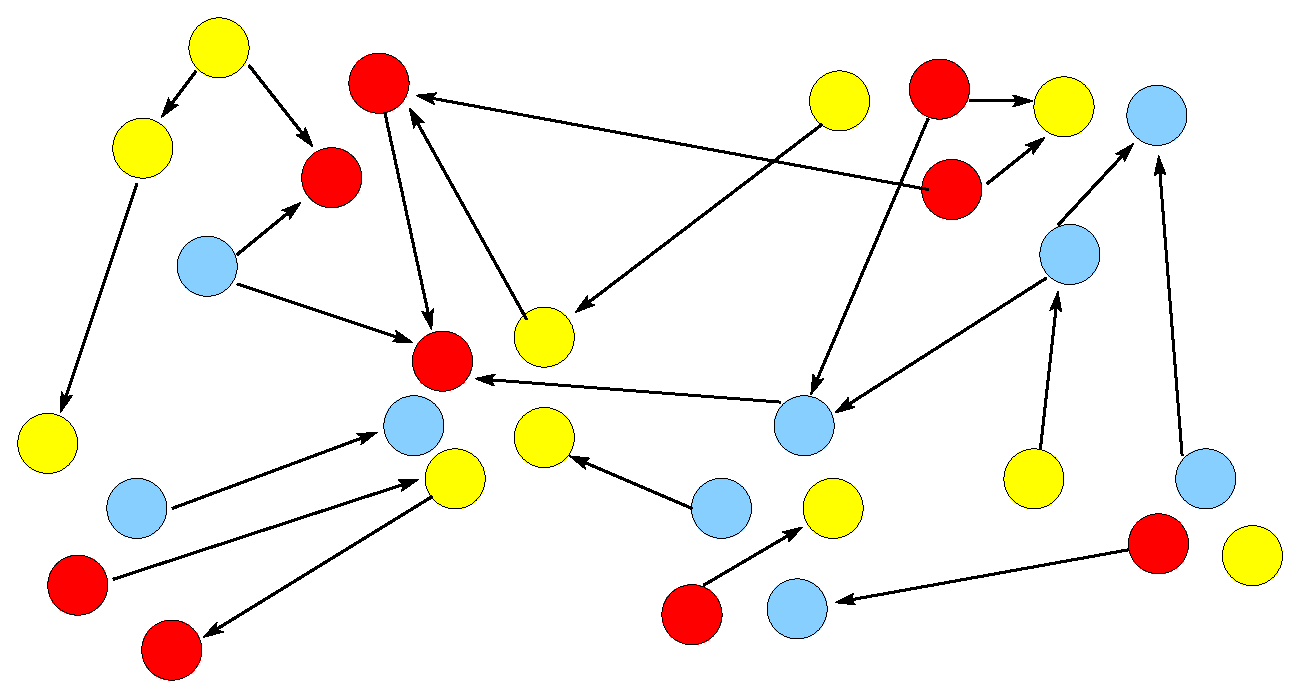
\includegraphics[width=0.45\linewidth]{gm.eps}  } 
\subfigure[second caption]{ 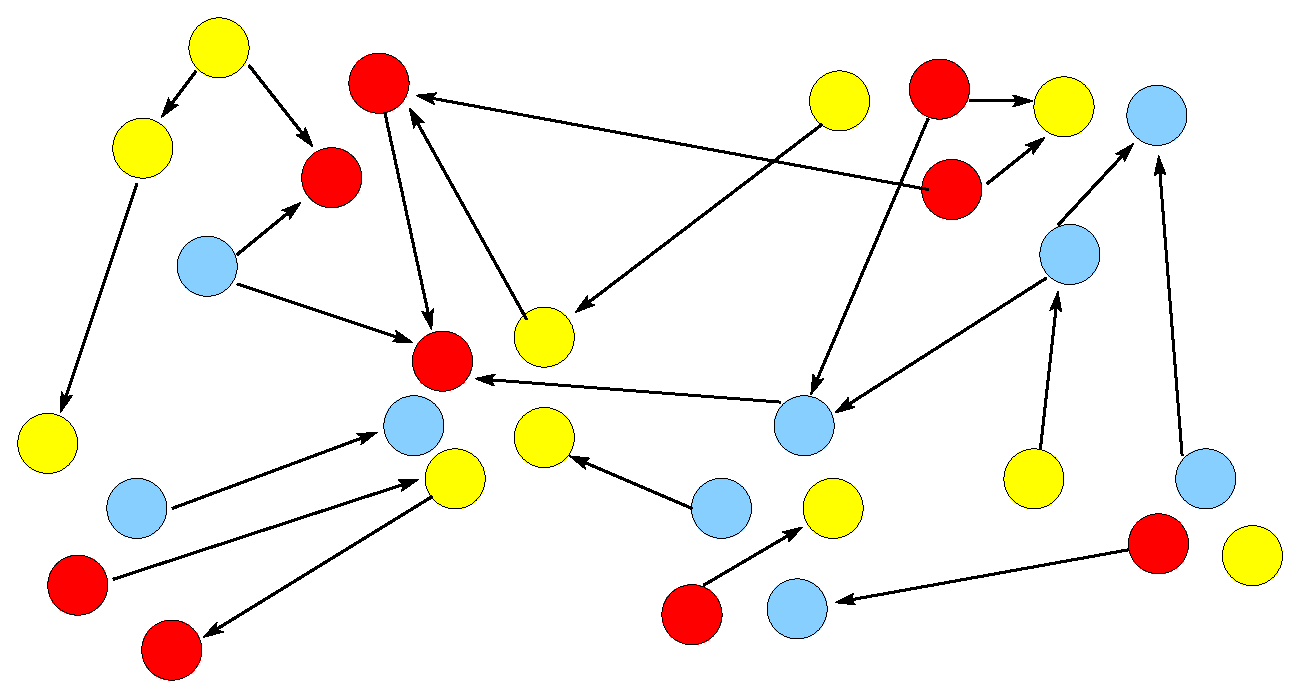
\includegraphics[width=0.45\linewidth]{gm.eps}  }
\caption{ตัวอย่างการใช้ subfigure}
\end{figure}

\subsection{การพิมพ์สมการ}
กรณีพิมพ์สมการมีทั้งที่แทรกในบรรทัด เช่น $y=Cx$ หรือการแยกเป็นบรรทัดใหม่
\begin{equation}
	F(s) = \int_0^\infty e^{-st} f(t) dt
\end{equation}

การใช้ package 'align' จะสามารถเขียนสัญลักษณ์ต่างๆ ได้มากกว่า 1 บรรทัด มีได้หลายคอลัมน์ และสามารถจัดเรียงตำแหน่งได้ด้วย เช่น
\begin{align}
    x    &= 2 \label{eq:x} \\
    y    &= 3 \label{eq:y} \\
    z    &= x \times y \nonumber \\
        &= p \label{eq:results}
\end{align}
การไม่ใส่หมายเลขสมการ สามารถใช้คำสั่ง \texttt{\nonumber} หรือ \texttt{notag} ได้ โดยปกติแล้วหากไม่ใส่อะไรเลย สมการทุกสมการจะมีหมายเลขกำกับเสมอ หลักการใส่เลขสมการคือ จะใส่เลขสมการก็ต่อเมื่อสมการนั้นจะถูกอ้างถึงในภายหลัง ดังนั้นการอ้างอึง (cross reference) สามารถทำได้โดยใช้คำสั่ง \texttt{ref} หรือ \texttt{eqref} กับ \texttt{label} ตัวอย่างเช่น สมการ~\eqref{eq:x} กล่าวไว้ว่า $x=2$

package 'eqnarray' ก็จะเป็นอีก environment หนึ่งที่ใช้เรียงสมการออกเป็น array

\begin{eqnarray}
\dot{x} &=& Ax + Bu \\
y &=& Cx+Du
\end{eqnarray}

ถ้าหากมีสมการหลายบรรทัดและต้องการเรียงในแนว center ให้ใช้ package 'gather'
\begin{gather}
y = \sum_{n=0}^100 0.5^n + \sin(2\pi n t) + \lim_{n \rightarrow \infty} \frac{\log n}{n} \\
z = \lim_{t \rightarrow \infty} e^{-st} g(t) 
\end{gather}

\subsection{การใส่เอกสารอ้างอิง}
รูปแบบการเขียนเอกสารอ้างอิง ให้อิงตามรูปแบบที่ใช้ในบทความวิชาการเดียวกันทั้งรายงาน การอ้างอิงถึงเอกสารต่างชนิดกัน (เช่น หนังสือ บทความที่ตีพิมพ์ในวารสารวิชาการ บทความที่นำเสนอในที่ประชุมวิชาการ วิทยานิพนธ์) จะมีรูปแบบการอ้างอิงที่ต่างกัน และเป็นไปตามความนิยมหรือมาตรฐานต่าง ๆ ตัวอย่างรูปแบบการอ้างอิงแบบหนึ่งที่เป็นที่นิยมใช้มากในสาขาวิศวกรรมไฟฟ้าคือ รูปแบบการอ้างอิงของ IEEE ตามเอกสาร

\url{https://ieee-dataport.org/sites/default/files/analysis/27/IEEE Citation Guidelines.pdf}

การเรียงลำดับรายการเอกสารอ้างอิงแบบ IEEE ให้เรียงตามการอ้างถึงในเนื้อหารายงาน (อ้างถึงก่อนใช้ตัวเลขน้อย อ้างถึงทีหลังใช้ตัวเลขที่มากกว่า) โดยรายการเอกสารอ้างอิงดังข้างต้น ต้องปรากฏอยู่ในเนื้อความภายในรายงานด้วย (ไม่ต้องใส่เอกสารอ้างอิงที่ไม่ได้มีการอ้างถึงในรายงาน)


เอกสารอ้างอิงจะทำได้โดยง่าย หากใช้ \texttt{bibtex} โดยหลักการคร่าวๆ คือต้องมีไฟล์ฐานข้อมูลของเอกสารอ้างอิง เก็บในรูปแบบ \texttt{file.bib} ซึ่งบรรจุรหัสของเอกสารอ้างอิงที่ผู้ใช้ตั้งเอง และรายละเอียดของเปเปอร์นั้นๆ (สร้างได้โดยง่ายจากการใช้ Google Scholar ช่วย) ตัวอย่างการใช้งานคือ การใช้คำสั่ง \texttt{cite} เมื่อต้องการจะอ้างถึงเอกสารนั้นๆ เช่น หลักการ system identification เบื้องต้นนั้นสามารถอ่านได้จาก~\cite{SoS:89} เป็นต้น

\bibliography{ref}
\bibliographystyle{ieeetr}

\section{ภาคผนวก (ถ้ามี)}
ภาคผนวกเป็นข้อความที่ไม่สามารถใส่ไว้ในเนื้อหาหลักได้ แต่สามารถทำให้ผู้อ่านเข้าใจรายละเอียดของโครงงานได้มากยิ่งขึ้น ในหัวข้อนี้ให้ใส่รายละเอียดหรือข้อมูลอื่นๆ ที่จำเป็น ซึ่งไม่สำคัญเท่ากับที่อยู่ในเนื้อหาหลัก เช่น

\begin{itemize}
    \item ทฤษฎีพื้นฐานเพิ่มเติม เพื่อให้ผู้อ่านเข้าใจวิธีการที่ใช้ในโครงงานได้ดีขึ้น แต่การไม่ใส่รายละเอียดนี้ต้องไม่ทำให้ผู้อ่านไม่สามารถติดตามหรือเข้าใจเนื้อหาหลักได้
    \item Data Sheet ของอุปกรณ์ที่เลือกใช้
    \item Specification ของฮาร์ดแวร์ต่างๆ
    \item Features ของซอฟต์แวร์ที่ใช้
    \item Source Code ของโปรแกรมที่ได้เขียนขึ้นมาเอง หรือดัดแปลงมา
    \item Device Characteristics ของชิ้นส่วนในโครงงาน
\end{itemize}

ภาคผนวกอาจแบ่งออกเป็นหลายส่วน ตามหัวข้อเรื่อง เช่น

\subsection{ภาคผนวก ก.}

\subsection{ภาคผนวก ข.}

\end{document}